\part{Lecture 12: Deterministic Policy Gradient Methods}
\title[RL Lecture 12]{Lecture 12: Deterministic Policy Gradient Methods}  
\date{}  
\frame{\titlepage} 

%%%%%%%%%%%%%%%%%%%%%%%%%%%%%%%%%%%%%%%%%%%%%%%%%%%%%%%%%%%%%%%%%%
\section{Deterministic gradient policy} 
%%%%%%%%%%%%%%%%%%%%%%%%%%%%%%%%%%%%%%%%%%%%%%%%%%%%%%%%%%%%%%%%%%
\begin{frame}
\frametitle{Table of contents}
\tableofcontents
\end{frame}

%%%%%%%%%%%%%%%%%%%%%%%%%%%%%%%%%%%%%%%%%%%%%%%%%%%%%%%%%%%%%
%% Background and Motivation %%
%%%%%%%%%%%%%%%%%%%%%%%%%%%%%%%%%%%%%%%%%%%%%%%%%%%%%%%%%%%%%
\frame{\frametitle{Background and motivation}
Recap on policy gradient so far:
\begin{itemize}
	\item The previously discussed policy functions and the policy gradient theorem were assuming stochastic polices. \pause
	\item The resulting on-policy algorithms may not provide top-class learning performance: \pause
	\begin{itemize}
		\item Non-guided exploration with step-by-step updates and
		\item Greedy actions only in the limit (i.e., infeasible long learning).  
	\end{itemize}\pause
\end{itemize}
\vspace{0.5cm}
The alternative:
\begin{itemize}
	\item Apply a deterministic policy with separate exploration. \pause
	\item Enable off-policy learning (with experience replay as a possible extension). \pause
	\item Hence, we will focus on a \hl{deterministic policy function}
	\begin{equation}
		\pi(\bm{x}, \bm{\theta}) = \mu(\bm{x}, \bm{\theta}) .
	\end{equation}
\end{itemize}
}

%%%%%%%%%%%%%%%%%%%%%%%%%%%%%%%%%%%%%%%%%%%%%%%%%%%%%%%%%%%%%
%% Deterministic Policy Gradient Theorem %%
%%%%%%%%%%%%%%%%%%%%%%%%%%%%%%%%%%%%%%%%%%%%%%%%%%%%%%%%%%%%%
\frame{\frametitle{Deterministic policy gradient (DPG) theorem}
\begin{theo}{Deterministic Policy Gradient}{determ_policy_gradient}
Given a metric $J(\bm{\theta})$ for the undiscounted episodic \eqref{eq:performance_metric_episodic} or continuing tasks \eqref{eq:performance_metric_continuing} and  a parameterizable policy $\mu(\bm{x},\bm{\theta})$ the deterministic policy gradient is
\begin{equation}
	\nabla_{\bm{\theta}} J(\bm{\theta}) = \El{\nabla_{\bm{\theta}} \mu(\bm{x},\bm{\theta}) \nabla_{\bm{u}} q(\bm{x},\bm{u})\vert_{\bm{u}=\mu(\bm{x})}}{\mu}.
	\label{eq:policy_gradient_theo_det}
\end{equation}
\end{theo}\pause
\begin{itemize}
\item Again, $q$ needs to be approximated using samples, e.g., implementing a critic via TD learning.\pause
\item It turns out that \eqref{eq:policy_gradient_theo_det} is also (approximately) valid in the off-policy case, i.e., if the sample distribution is obtained from a behavior policy.\pause  
\item Proof can be found in \href{http://proceedings.mlr.press/v32/silver14.pdf}{D. Silver et al., \textit{Deterministic Policy Gradient Algorithms}, International Conference on Machine Learning, 2014}

\end{itemize}
}

%%%%%%%%%%%%%%%%%%%%%%%%%%%%%%%%%%%%%%%%%%%%%%%%%%%%%%%%%%%%%
%% Exploration %%
%%%%%%%%%%%%%%%%%%%%%%%%%%%%%%%%%%%%%%%%%%%%%%%%%%%%%%%%%%%%%
\frame{\frametitle{Exploration with a deterministic policy}
\begin{itemize}
	\item If the DPG approach is applied on-policy there is no inherent exploration.
	\item How to learn something?\pause
	\begin{itemize}
		\item The environment itself is sufficiently noisy (random impacts, measurement noise).\pause
		\item Or we have to add noise to the actions, i.e., making the approach off-policy.\pause
		\item Hence, utilizing a behavior policy is also possible.\pause
	\end{itemize}
	\item That additional action noise could be:
	\begin{itemize}
		\item Simple Gaussian noise or\pause
		\item a shaped noise process like a discrete-time Ornstein-Uhlenbeck (OU) process
		\begin{equation*}
			\nu_{k+1} = \lambda \nu_k+ \sigma \epsilon_k
		\end{equation*}
		where $\nu_k$ is the OU noise output, $0 < \lambda < 1$ is a  smoothing factor and $\sigma$ is the variance scaling a standard Gaussian sequence (no mean) $\epsilon_k$. 
	\end{itemize}
\end{itemize}
}

%%%%%%%%%%%%%%%%%%%%%%%%%%%%%%%%%%%%%%%%%%%%%%%%%%%%%%%%%%%%%
%% Algorithmic Implementation: Deterministic Actor-Critic %%
%%%%%%%%%%%%%%%%%%%%%%%%%%%%%%%%%%%%%%%%%%%%%%%%%%%%%%%%%%%%%
\frame{\frametitle{Algo. implementation: deterministic actor-critic}
\setlength{\algomargin}{0.5em}
\begin{algorithm}[H]
\small
\SetKwInput{Input}{input} 
\SetKwInput{Output}{output}
\SetKwInput{Init}{init}
\SetKwInput{Param}{parameter}
\Input{a differentiable deterministic policy function $\mu(\bm{x},\bm{\theta})$}
\Input{a differentiable action-value function $\hat{q}(\bm{x},\bm{u},\bm{w})$}
\Param{step sizes $\{\alpha_{w}, \alpha_{\theta}\}\in\left\{\mathbb{R}|0<\alpha<1\right\}$}
\Init{parameter vectors $\bm{w}\in\mathbb{R}^{\zeta}$ and $\bm{\theta}\in\mathbb{R}^d$ arbitrarily}
 \For{$j=1,2,\ldots,$ episodes}{
		initialize $\bm{x}_0$\; 
		\For{$k=0,1,\ldots, T-1$ time steps}{
			$\bm{u}_k \leftarrow$ apply from $\mu(\bm{x}_k, \bm{\theta})$ w/wo noise or from behavior policy\;
			observe $\bm{x}_{k+1}$ and $r_{k+1}$\;
			choose $\bm{u}'$ from $\mu(\bm{x}_{k+1}, \bm{\theta})$\;
			$\delta \leftarrow r_{k+1} + \gamma \hat{q}(\bm{x}_{k+1}, \bm{u}', \bm{w})- \hat{q}(\bm{x}_k, \bm{u}_k, \bm{w})$\;
			$\bm{w} \leftarrow \bm{w}+\alpha_w\delta\nabla_{\bm{w}}\hat{q}(\bm{x}_k, \bm{u}_k, \bm{w})$\;
			$\bm{\theta} \leftarrow \bm{\theta} + \alpha_{\theta} \gamma^k \nabla_{\bm{\theta}}\mu(\bm{x}_k,\bm{\theta})\nabla_{\bm{u}}\hat{q}(\bm{x}_k, \bm{u}_k, \bm{w})\vert_{\bm{u}=\mu(\bm{x})}$\; 
		}
	}
\caption{Deterministic actor-critic for episodic tasks using SARSA(0) targets applicable on- and off-policy (output: parameter vector $\bm{\theta}^*$ for $\mu^*(\bm{x},\bm{\theta}^*)$) and $\bm{w}^*$ for $\hat{q}^*(\bm{x}, \bm{u}, \bm{w}^*))$}
\label{algo:det_actor_critic_Sarsa0_episode}
\end{algorithm}
}


%%%%%%%%%%%%%%%%%%%%%%%%%%%%%%%%%%%%%%%%%%%%%%%%%%%%%%%%%%%%%
%% Exemplary Comparison to Stochastic Policy Gradient %%
%%%%%%%%%%%%%%%%%%%%%%%%%%%%%%%%%%%%%%%%%%%%%%%%%%%%%%%%%%%%%
\frame{\frametitle{Exemplary comparison to stochastic policy gradient}
\begin{itemize}
	\item DPG-based approach uses compatible function approximation, i.e., suitable linear $\hat{q}$ estimation. A fixed Gaussian behavior policy is applied for exploration. 
	\item SAC uses a Gaussian policy with linear function approximation.
\end{itemize}
\begin{figure}
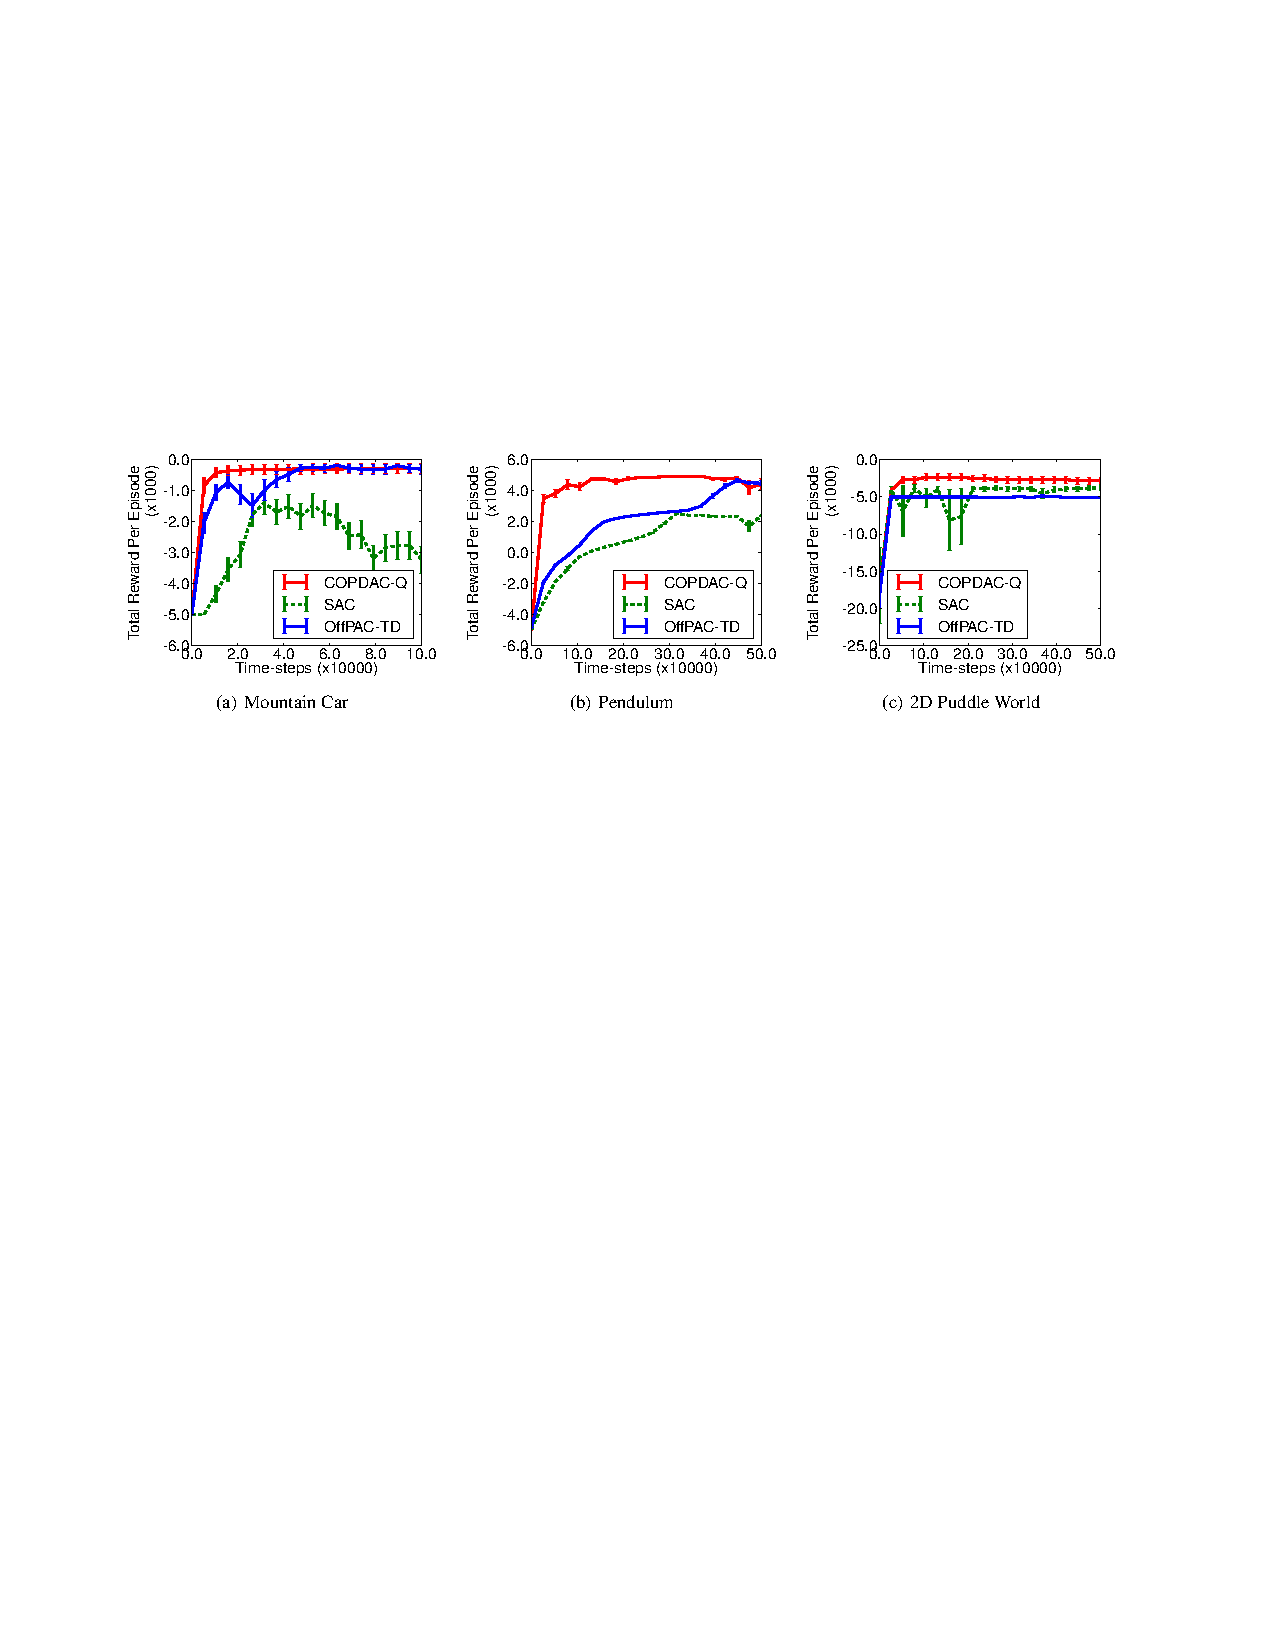
\includegraphics[width=11cm]{fig/lec12/SLH_Benchmarks.pdf}
\caption{Comparison of stochastic on-policy actor-critic (SAC), stochastic off-policy actor-critic (OffPAC), and deterministic off-policy
actor-critic (COPDAC) on continuous-action reinforcement learning (source: D. Silver et al., \textit{Deterministic Policy Gradient Algorithms}, International Conference on Machine Learning, 2014)}
\label{fig:SLH_Benchmarks}
\end{figure}
}

%%%%%%%%%%%%%%%%%%%%%%%%%%%%%%%%%%%%%%%%%%%%%%%%%%%%%%%%%%%%%%%%%%
\section{Deep deterministic policy gradient (DDPG)} 
%%%%%%%%%%%%%%%%%%%%%%%%%%%%%%%%%%%%%%%%%%%%%%%%%%%%%%%%%%%%%%%%%%
\begin{frame}
\frametitle{Table of contents}
\tableofcontents[currentsection]
\end{frame}

%%%%%%%%%%%%%%%%%%%%%%%%%%%%%%%%%%%%%%%%%%%%%%%%%%%%%%%%%%%%%
%% Motivation / General Idea %%
%%%%%%%%%%%%%%%%%%%%%%%%%%%%%%%%%%%%%%%%%%%%%%%%%%%%%%%%%%%%%
\frame{\frametitle{Motivation / general idea}
\begin{itemize}
	\item The upcoming \hl{deep deterministic policy gradient (DDPG)} algorithm was very much inspired by the successes of DQNs (cf. \algoref{algo:DQN} and landmark \href{https://www.nature.com/articles/nature14236?wm=book_wap_0005}{paper by Mnih et al.}) on discrete action spaces.\pause
	\item However, \hl{DQNs are not directly applicable to (quasi-)continuous action spaces}.\pause
	\item Recall the incremental $Q$-learning  equation using function approximation
	\begin{equation*}
	 \bm{w} \leftarrow \bm{w} + \alpha\left[r+\gamma \max_u \hat{q}(\bm{x}', u, \bm{w}) - \hat{q}(\bm{x}, u, \bm{w})\right]\nabla_{\bm{w}} \hat{q}(\bm{x}, u, \bm{w}).
 \end{equation*}
	\item For every policy inference and updating step we need to find $\max_u \hat{q}(\bm{x}', u, \bm{w})$.\pause 
	\item If $u\in\mathcal{U}\subset\mathbb{Z}$ (i.e., using integer-encoded actions) is a sufficiently small discrete set, that is straightforward by an exhaustive search.\pause
	\item In contrast, if $\bm{u}\in\mathcal{U}\subset\mathbb{R}^m$ is a (quasi-)continuous variable solving $\max_{\bm{u}} \hat{q}(\bm{x}', \bm{u}, \bm{w})$  requires an own \hl{optimization routine} which is computationally expensive if we use nonlinear function approximation. 
\end{itemize}
}

%%%%%%%%%%%%%%%%%%%%%%%%%%%%%%%%%%%%%%%%%%%%%%%%%%%%%%%%%%%%%
%% The Deterministic Policy Trick %%
%%%%%%%%%%%%%%%%%%%%%%%%%%%%%%%%%%%%%%%%%%%%%%%%%%%%%%%%%%%%%
\frame{\frametitle{The deterministic policy trick}
\begin{itemize}
	\item When using a greedy, deterministic policy $\bm{\pi}(\bm{x}, \bm{\theta}) = \bm{\mu}(\bm{x}, \bm{\theta})$ we can utilize it to approximate
	\begin{equation}
		\max_{\bm{u}} \hat{q}(\bm{x}', \bm{u}, \bm{w}) \approx \hat{q}(\bm{x}', \bm{\mu}(\bm{x}', \bm{\theta}), \bm{w}).
	\end{equation}
	\item Hence, we can obtain explicit $Q$-learning targets for continuous actions when using a deterministic policy.\pause 
	\item For improving the policy we reuse the deterministic policy gradient theorem in an off-policy fashion
	\begin{equation}
	\nabla_{\bm{\theta}} J(\bm{\theta}) = \El{\nabla_{\bm{\theta}} \bm{\mu}(\bm{X},\bm{\theta}) \nabla_{\bm{u}} q(\bm{X},\bm{U})\left|\bm{U}=\bm{\mu}(\bm{X}, \bm{\theta})\right.}{b}
\end{equation}
given a behavior policy $b(\bm{u}|\bm{x})$.
\end{itemize}
}

%%%%%%%%%%%%%%%%%%%%%%%%%%%%%%%%%%%%%%%%%%%%%%%%%%%%%%%%%%%%%
%% DDPG $\approx$ DQN + DPG %%
%%%%%%%%%%%%%%%%%%%%%%%%%%%%%%%%%%%%%%%%%%%%%%%%%%%%%%%%%%%%%
\frame{\frametitle{DDPG $\approx$ DQN + DPG}
\begin{itemize}
	\item Hence, we can consider the DDPG approach as a combination of DQN + DPG rendering it an \hl{actor-critic off-policy approach for continuous state and action spaces}.\pause
	\item Similarly to DQN we will introduce \hl{several 'tweaks'} to stabilize and improve the DDPG learning process.\pause	
\end{itemize}
\vspace{0.25cm}
\hl{Tweak \#1}: experience replay buffer
\begin{itemize}
	\item We store $\left\langle \bm{x}, \bm{u}, r, \bm{x}'\right\rangle$ in $\bm{\mathcal{D}}$ after each transition step.\pause
	\item The replay buffer $\bm{\mathcal{D}}$ is of limited capacity, i.e., it discards the oldest data sample when updating once it is full (ring memory).\pause
	\item This allows us to improve the $Q$-learning critic minimizing the mean-squared Bellman error (MSBE):
	\begin{equation}
	\label{eq:MSBE_DDPG}
		\mathcal{L}(\bm{w}) = \left[\left(r+ \gamma q(\bm{x}',\bm{\mu}(\bm{x}',\bm{\theta}),\bm{w})\right) - q(\bm{x},\bm{u},\bm{w}) \right]^2_{\bm{\mathcal{D}}} .
	\end{equation}
\end{itemize}
}

%%%%%%%%%%%%%%%%%%%%%%%%%%%%%%%%%%%%%%%%%%%%%%%%%%%%%%%%%%%%%
%% Additional DDPG Tweaks (1) %%
%%%%%%%%%%%%%%%%%%%%%%%%%%%%%%%%%%%%%%%%%%%%%%%%%%%%%%%%%%%%%
\frame{\frametitle{Additional DDPG tweaks (1)}
\hl{Tweak \#2}: target networks
\begin{itemize}
	\item Similar to DQN we introduce a (delayed) target network to estimate the $Q$-learning target $$r+ \gamma q(\bm{x}',\bm{\mu}(\bm{x}',\bm{\theta}),\bm{w})$$ since it depends on the same parameters $\bm{w}$ which we want to update.\pause
	\item Hence, the target network's purpose it to mimic the generation of i.i.d. data as the ground truth to minimize \eqref{eq:MSBE_DDPG}.\pause
	\item Since the policy parameters $\bm{\theta}$ are also part of the target calculation it turns out that an additional policy target network is also beneficial to stabilize the $Q$-learning.\pause
	\item In contrast to the classical DQN implementation, the original DDPG algorithm does not perform periodically hard target network updates but continuous ones using a low-pass filter characteristic
	\begin{equation}
		\bm{w}^{-} \leftarrow (1-\tau)\bm{w}^{-}+\tau\bm{w}, \quad \bm{\theta}^{-} \leftarrow (1-\tau)\bm{\theta}^{-}+\tau\bm{\theta}
	\end{equation}
	with $\tau$ representing the equivalent filter constant (hyperparameter).
\end{itemize}
}

%%%%%%%%%%%%%%%%%%%%%%%%%%%%%%%%%%%%%%%%%%%%%%%%%%%%%%%%%%%%%
%% Additional DDPG Tweaks (2) %%
%%%%%%%%%%%%%%%%%%%%%%%%%%%%%%%%%%%%%%%%%%%%%%%%%%%%%%%%%%%%%
\frame{\frametitle{Additional DDPG tweaks (2)}
\hl{Tweak \#3}: mini-batch sampling
\begin{itemize}
	\item Given a sufficiently filled memory $\bm{\mathcal{D}}$ and the target networks parametrized by $\bm{w}^{-}$ and $\bm{\theta}^{-}$ we draw uniformly distributed mini-batch samples $\bm{\mathcal{D}}_b$ from $\bm{\mathcal{D}}$.\pause
	\item The actual $Q$-learning is then based on the loss
		\begin{equation}
		\label{eq:Loss_DDPG}
				\mathcal{L}(\bm{w}) = \left[\left(r+ \gamma q(\bm{x}',\bm{\mu}(\bm{x}',\bm{\theta}^{-}),\bm{w}^{-})\right) - q(\bm{x},\bm{u},\bm{w}) \right]^2_{\bm{\mathcal{D}}_b} \, .
	\end{equation}
\end{itemize}\pause
\hl{Tweak \#4}: batch normalization
\begin{itemize}
	\item Minimizing \eqref{eq:Loss_DDPG} is a supervised learning step within the DDPG.\pause
	\item The \href{https://arxiv.org/abs/1509.02971}{original DDPG paper by Lillicrap et al.} back in 2015/16 suggested to use batch normalization, i.e., re-centering and re-scaling the inputs of each layer in an ANN.\pause
	\item This idea of batch normalization was presented at that time shortly before by Ioffe and Szegedy (cf. \href{http://proceedings.mlr.press/v37/ioffe15.html}{original paper}).\pause
	\item Today's perspective: stick to the current state-of-the-art supervised ML algorithms for top-class $Q$-learning stability and speed (which are normally well-covered in popular supervised ML toolboxes). 
\end{itemize}
}

%%%%%%%%%%%%%%%%%%%%%%%%%%%%%%%%%%%%%%%%%%%%%%%%%%%%%%%%%%%%%
%% Additional DDPG Tweaks (3) %%
%%%%%%%%%%%%%%%%%%%%%%%%%%%%%%%%%%%%%%%%%%%%%%%%%%%%%%%%%%%%%
\frame{\frametitle{Additional DDPG tweaks (3)}
\setcounter{footnote}{0}
\hl{Tweak \#5}: exploration
\begin{itemize}
	\item Since our policy is deterministic we require an exploratory behavior policy.\pause
	\item Similar to DPG the standard approach is to add noise to the greedy actions, e.g., again from an Ornstein-Uhlenbeck (OU) process
		\begin{equation*}
			\bm{u}_k\sim\bm{b}(\bm{u}|\bm{x}_k)=\bm{\mu}(\bm{x}_k,\bm{\theta}_k)+\bm{\nu}_{k},\quad \bm{\nu}_{k}= \lambda \bm{\nu}_{k-1}+ \sigma \bm{\epsilon}_{k-1}.
		\end{equation*}\pause
		\item One might also add a schedule for $\lambda$ and $\sigma$ along the training procedure, e.g., starting with significant noise levels (increased exploration) while reducing it over time (focusing exploitation)\footnote{Please note that this 'lambda' is not related to TD($\lambda$), SARSA($\lambda$), etc. Here, it is representing the stiffness of the OU noise process.}.\pause  
	\item However, many other behavior policies are possible, e.g., using model or expert-based guidance.
\end{itemize}
}

%%%%%%%%%%%%%%%%%%%%%%%%%%%%%%%%%%%%%%%%%%%%%%%%%%%%%%%%%%%%%
%% Summary of DQN Working Principle  (2)%%
%%%%%%%%%%%%%%%%%%%%%%%%%%%%%%%%%%%%%%%%%%%%%%%%%%%%%%%%%%%%%
\frame{\frametitle{Visual summary of DDPG working principle}
\begin{figure}
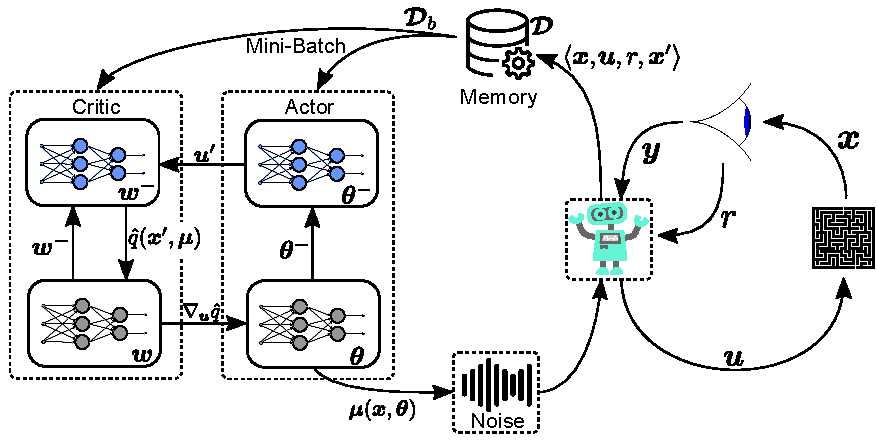
\includegraphics[height=5.75cm]{fig/lec12/DDPG.pdf}
\caption{DDPG structure from a bird's-eye perspective (derivative work of \figref{fig:RL_Wiki} and \href{https://commons.wikimedia.org/wiki/File:Multi-Layer_Neural_Network-Vector.svg?uselang=de}{wikipedia.org}, \href{https://creativecommons.org/publicdomain/zero/1.0/deed.en}{CC0 1.0})}
\label{fig:DDPG}
\end{figure}
}	

%%%%%%%%%%%%%%%%%%%%%%%%%%%%%%%%%%%%%%%%%%%%%%%%%%%%%%%%%%%%%
%% Algorithmic Implementation: DDPG %%
%%%%%%%%%%%%%%%%%%%%%%%%%%%%%%%%%%%%%%%%%%%%%%%%%%%%%%%%%%%%%
\frame{\frametitle{Algo. implementation: DDPG}
\setlength{\algomargin}{0.5em}
\begin{algorithm}[H]
\small
\SetKwInput{Input}{input} 
\SetKwInput{Output}{output}
\SetKwInput{Init}{init}
\SetKwInput{Param}{parameter}
\Input{diff. deterministic policy function $\bm{\mu}(\bm{x},\bm{\theta})$ and action-value function $\hat{q}(\bm{x},\bm{u},\bm{w})$}
\Param{step sizes and filter constant $\{\alpha_{w}, \alpha_{\theta}, \tau\}\in\left\{\mathbb{R}|0<\alpha, \tau<1\right\}$}
\Init{weights $\bm{w}=\bm{w}^{-}\in\mathbb{R}^{\zeta}$ and $\bm{\theta}=\bm{\theta}^{-}\in\mathbb{R}^d$ arbitrarily, memory $\bm{\mathcal{D}}$}\pause
 \For{$j=1,2,\ldots,$ episodes}{
		initialize $\bm{x}_0$\; 
		\For{$k=0,1,\ldots, T-1$ time steps}{
			$\bm{u}_k \leftarrow$ apply from $\bm{\mu}(\bm{x}_k, \bm{\theta})$ w/wo noise or from behavior policy\;
			observe $\bm{x}_{k+1}$ and $r_{k+1}$\;
			store tuple $\left\langle \bm{x}_k, \bm{u}_k, r_{k+1}, \bm{x}_{k+1}\right\rangle$ in $\bm{\mathcal{D}}$\;\pause
			sample mini-batch $\bm{\mathcal{D}}_b$ from $\bm{\mathcal{D}}$ (after initial memory warmup)\;
			\For(calculate $Q$-targets){$i=1,\ldots,b$ samples}{
				\lIf{$\bm{x}_{i+1}$ is terminal}{$y_i=r_{i+1}$}
				\lElse{$y_i= r_{i+1}+ \gamma \hat{q}(\bm{x}_{i+1},\bm{\mu}(\bm{x}_{i+1},\bm{\theta}^{-}),\bm{w}^{-})$}
			}\pause
			fit $\bm{w}$ on loss $\mathcal{L}(\bm{w})=[y - \hat{q}(\bm{x}, \bm{u}, \bm{w})]^2_{\bm{\mathcal{D}}_b}$ with step size $\alpha_{w}$\;\pause
			$\bm{\theta} \leftarrow \bm{\theta} + \alpha_{\theta} [\nabla_{\bm{\theta}}\bm{\mu}(\bm{x},\bm{\theta})\nabla_{\bm{u}}\hat{q}(\bm{x}, \bm{u}, \bm{w})\vert_{\bm{u}=\bm{\mu}_{\bm{\theta}}(\bm{x})}]_{\bm{\mathcal{D}}_b}$\;\pause 
			Update target net. $\bm{w}^{-} \leftarrow (1-\tau)\bm{w}^{-}+\tau\bm{w}, \,\, \bm{\theta}^{-} \leftarrow (1-\tau)\bm{\theta}^{-}+\tau\bm{\theta}$\;
		}
	}
\caption{Deep deterministic policy gradient (output: parameter vectors $\bm{\theta}^*$ for $\bm{\mu}^*(\bm{x},\bm{\theta}^*)$) and $\bm{w}^*$ for $\hat{q}^*(\bm{x}, \bm{u}, \bm{w}^*))$}
\label{algo:DDPG}
\end{algorithm}
}

%%%%%%%%%%%%%%%%%%%%%%%%%%%%%%%%%%%%%%%%%%%%%%%%%%%%%%%%%%%%%%%%%%
\section{Twin delayed deep deterministic policy gradient (TD3)} 
%%%%%%%%%%%%%%%%%%%%%%%%%%%%%%%%%%%%%%%%%%%%%%%%%%%%%%%%%%%%%%%%%%
\begin{frame}
\frametitle{Table of contents}
\tableofcontents[currentsection]
\end{frame}

%%%%%%%%%%%%%%%%%%%%%%%%%%%%%%%%%%%%%%%%%%%%%%%%%%%%%%%%%%%%%
%% Overestimation Bias %%
%%%%%%%%%%%%%%%%%%%%%%%%%%%%%%%%%%%%%%%%%%%%%%%%%%%%%%%%%%%%%
\frame{\frametitle{Overestimation bias}
\begin{itemize}
	\item For $Q$-learning in the tabular case we have already discussed the \hl{maximization bias} (cf. \figref{Double_Learning_Example}) issue.\pause
	\item Recap: Due to the greedy policy targets, $\hat{q}$ was overestimated when calculated using sampled values of stochastic MDPs.\pause
	\item Additional problem when applying function approximation: the estimator itself introduces additional variance during the learning process which represents another source of the maximization bias problem.\pause
\end{itemize}
\begin{block}{}
This issue is already known in the DQN context (cf. \algoref{algo:DQN}). Similar to the tabular case, \hl{double DQN} introduces a second $Q$-network counteracting the overestimation issue (cf. \href{https://arxiv.org/pdf/1509.06461.pdf}{paper by van Hasselt et al.}).
\end{block}\pause
However, we did not address this possible problem in an actor-critic context using function approximation (e.g., DDPG). 
}

%%%%%%%%%%%%%%%%%%%%%%%%%%%%%%%%%%%%%%%%%%%%%%%%%%%%%%%%%%%%%
%% Overestimation Bias in Actor-Critic Approaches (1) %%
%%%%%%%%%%%%%%%%%%%%%%%%%%%%%%%%%%%%%%%%%%%%%%%%%%%%%%%%%%%%%
\frame{\frametitle{Overestimation bias in actor-critic approaches (1)}
\begin{itemize}
	\item It turns out that the overestimation bias is also an issue for actor-critic methods\footnote[1]{Source: S. Fujimoto et al., \textit{Addressing Function Approximation Error in Actor-Critic Methods}, \href{https://arxiv.org/abs/1802.09477}{https://arxiv.org/abs/1802.09477}, 2018}.\pause
	\item Consider an actor-critic policy with the current policy parameters $\bm{\theta}$.\pause
	\item Let $\tilde{\bm{\theta}}$ define the parameters from the actor update induced by the maximization of the approximate critic $\hat{q}_{\bm{w}}(\bm{x}, \bm{u})$. \pause
	\item Let $\bm{\theta}^*$ be the parameters from the hypothetical actor update w.r.t. the true underlying value function $q^{\bm{\pi}}(\bm{x}, \bm{u})$.\pause
	\item Then, we perform the policy update
	\begin{equation}
\begin{aligned}
\tilde{\bm{\theta}} &= \bm{\theta} + \frac{\alpha}{Z_1} \El{\nabla_{\bm{\theta}} \pi_{\bm{\theta}}(\bm{X}) \nabla_{\bm{u}} \hat{q}_{\bm{w}}(\bm{X},\bm{U})\left|\bm{U}=\bm{\pi}_{\bm{\theta}}(\bm{X})\right.}{\pi},\\
\bm{\theta}^* &= \bm{\theta} + \frac{\alpha}{Z_2} \El{\nabla_{\bm{\theta}} \pi_{\bm{\theta}}(\bm{X}) \nabla_{\bm{u}} q^{\bm{\pi}}(\bm{X},\bm{U})\left|\bm{U}=\bm{\pi}_{\bm{\theta}}(\bm{X})\right.}{\pi},
\end{aligned}
\end{equation} 
where $Z_1$ and $Z_2$ normalize the gradient such that $Z^{-1}||\El{\cdot}{}|| = 1$.
\end{itemize}	
}

%%%%%%%%%%%%%%%%%%%%%%%%%%%%%%%%%%%%%%%%%%%%%%%%%%%%%%%%%%%%%
%% Overestimation Bias in Actor-Critic Approaches (2) %%
%%%%%%%%%%%%%%%%%%%%%%%%%%%%%%%%%%%%%%%%%%%%%%%%%%%%%%%%%%%%%
\frame{\frametitle{Overestimation bias in actor-critic approaches (2)}
\begin{itemize}
	\item Lets denote $\tilde{\bm{\pi}}$ and $\bm{\pi}^*$ as the policies with updated parameters $\tilde{\bm{\theta}}$ and $\bm{\theta}^*$ respectively.\pause
	\item As the gradient direction is a local maximizer, there exists $\epsilon_1$ sufficiently small such that if $\alpha \leq \epsilon_1$ then the \emph{approximate} value of $\tilde{\bm{\pi}}$ will be bounded below by the \emph{approximate} value of $\bm{\pi}^*$:
\begin{equation} \label{eq:approx_q_TD3}
\E{\hat{q}_{\bm{w}}(\bm{X}, \tilde{\bm{\pi}}(\bm{X}))} \geq \E{\hat{q}_{\bm{w}}(\bm{X}, \bm{\pi}^*(\bm{X}))}.
\end{equation}\pause
\item Conversely, there exists $\epsilon_2$ sufficiently small such that if $\alpha \leq \epsilon_2$ then the \emph{true} value of $\tilde{\bm{\pi}}$ will be bounded above by the \emph{true} value of $\bm{\pi}^*$:
\begin{equation} \label{eq:true_q_TD3}
\E{q^{\bm{\pi}}(\bm{X}, \bm{\pi}^*(\bm{X}))} \geq \E{q^{\bm{\pi}}(\bm{X}, \tilde{\bm{\pi}}(\bm{X}))}.
\end{equation}\pause
\item In other words: if the approximate and true critics differ from each other, the according policy gradient updates cannot lead to better policy updates of the respective other framework.  
\end{itemize}	
}

%%%%%%%%%%%%%%%%%%%%%%%%%%%%%%%%%%%%%%%%%%%%%%%%%%%%%%%%%%%%%
%% Overestimation Bias in Actor-Critic Approaches (3) %%
%%%%%%%%%%%%%%%%%%%%%%%%%%%%%%%%%%%%%%%%%%%%%%%%%%%%%%%%%%%%%
\frame{\frametitle{Overestimation bias in actor-critic approaches (3)}
\begin{itemize}
	\item If the expected, estimated action value will be at least as large as the \textit{true} action value w.r.t. $\bm{\theta}^*$
	\begin{equation}
  \E{\hat{q}_{\bm{w}}(\bm{X}, \bm{\pi}^*(\bm{X}))} \geq \E{q^{\bm{\pi}}(\bm{X}, \bm{\pi}^*(\bm{X}))}, 
\end{equation}\pause
then \eqref{eq:approx_q_TD3} and \eqref{eq:true_q_TD3} imply 
	\begin{equation}
  \E{\hat{q}_{\bm{w}}(\bm{X}, \tilde{\bm{\pi}}(\bm{X}))} \geq \E{q^{\bm{\pi}}(\bm{X}, \tilde{\bm{\pi}}(\bm{X}))}
\end{equation}
	with a sufficiently small $\alpha<\min\{\epsilon_1, \epsilon_2\}$.\pause
	\item Hence, the \hl{maximization bias is also present in actor-critic} updates.\pause
	\item It can add up over several estimation updates and, therefore, may lead to suboptimal policy updates.\pause
	\item A proof for unnormalized gradients can be also found in S. Fujimoto et al., \textit{Addressing Function Approximation Error in Actor-Critic Methods}, 2018.
\end{itemize}	
}

%%%%%%%%%%%%%%%%%%%%%%%%%%%%%%%%%%%%%%%%%%%%%%%%%%%%%%%%%%%%%
%% Overestimation Example for DDPG%%
%%%%%%%%%%%%%%%%%%%%%%%%%%%%%%%%%%%%%%%%%%%%%%%%%%%%%%%%%%%%%
\frame{\frametitle{Overestimation example for DDPG}
\vspace{0.75cm}
\begin{figure}
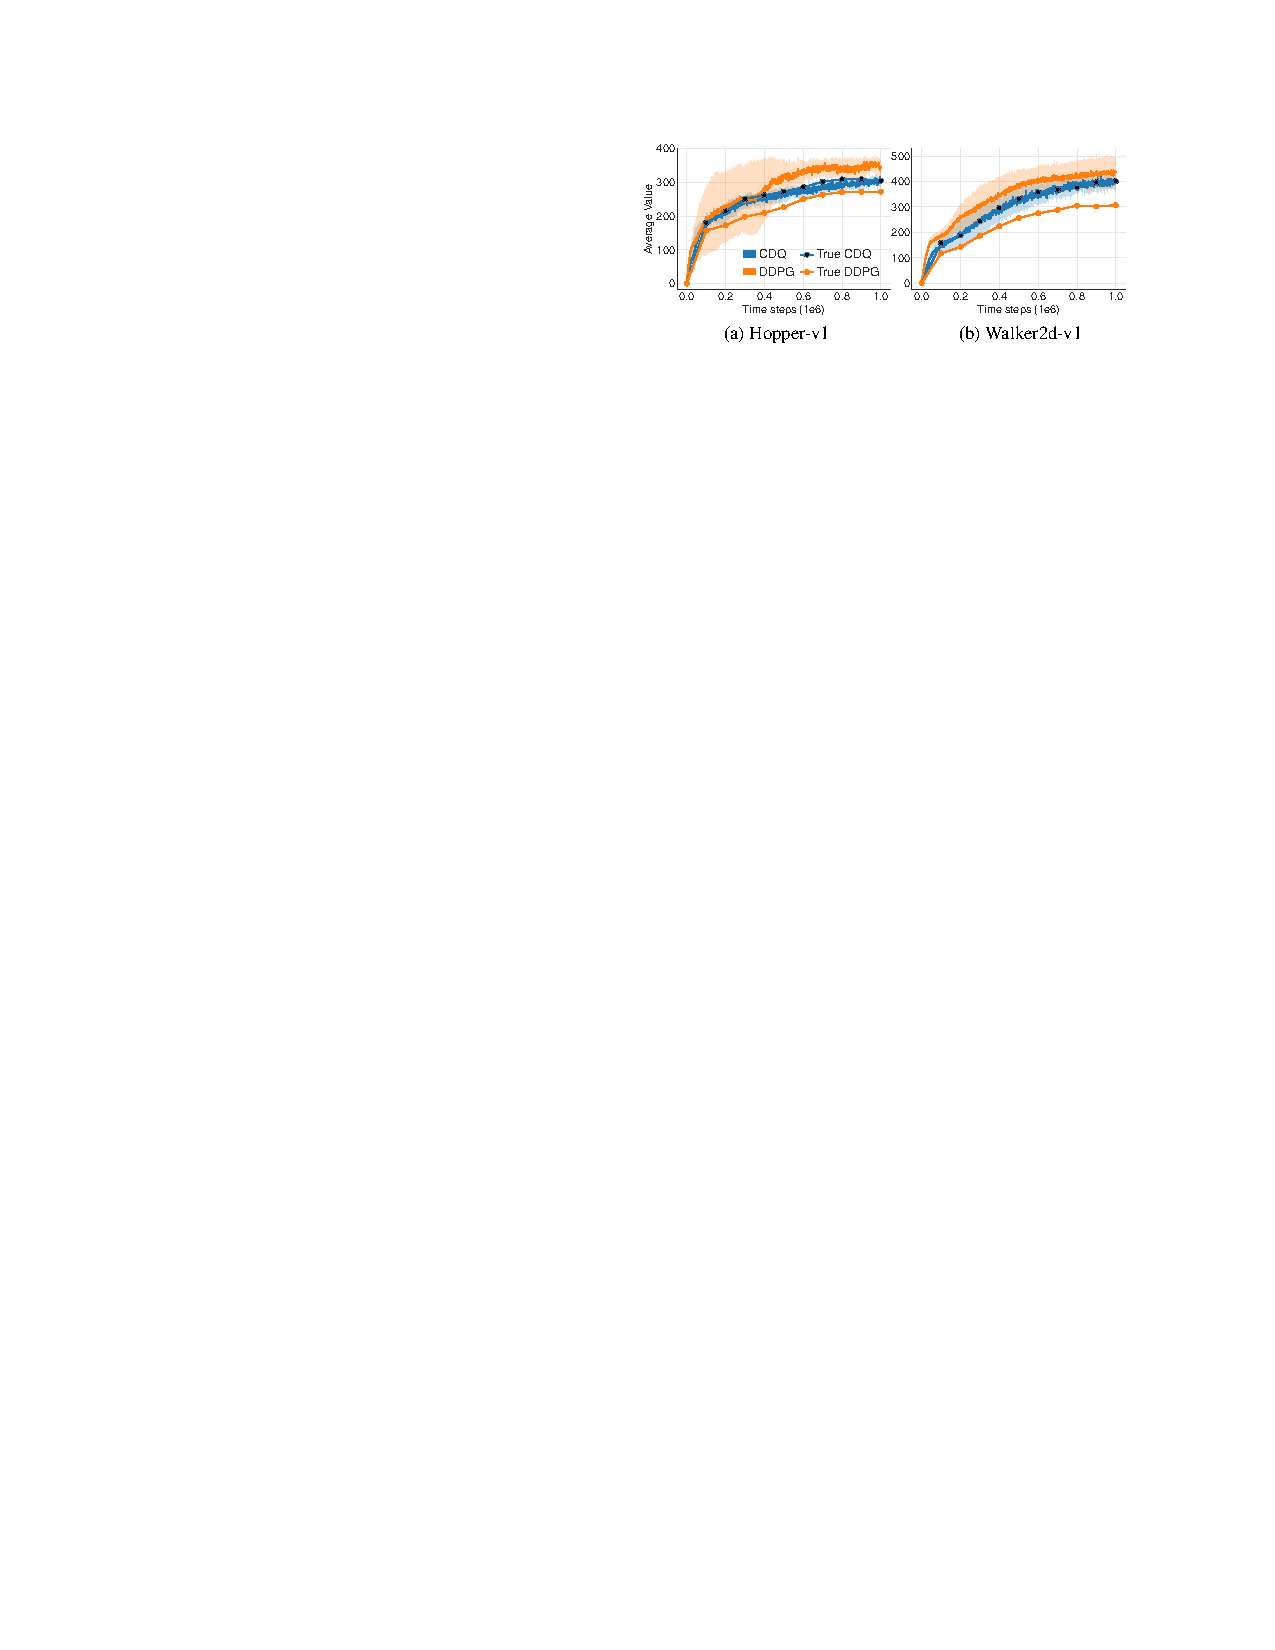
\includegraphics[height=4cm]{fig/lec12/DDPG_Overestimation.pdf}
\caption{Comparison of true and estimated values averaged over 10000 states in two robotic examples from \href{https://gym.openai.com/envs/\#mujoco}{OpenAI Gym}. Estimated values originate from the approximate DDPG critic while the true values are based on the average discounted return over 1000 episodes following the current policy, starting from states sampled from the replay buffer (source: S. Fujimoto et al., \textit{Addressing Function Approximation Error in Actor-Critic Methods}, 2018.}
\label{fig:DDPG_Overestimation}
\end{figure}
}	

%%%%%%%%%%%%%%%%%%%%%%%%%%%%%%%%%%%%%%%%%%%%%%%%%%%%%%%%%%%%%
%% Overestimation Example for DDPG%%
%%%%%%%%%%%%%%%%%%%%%%%%%%%%%%%%%%%%%%%%%%%%%%%%%%%%%%%%%%%%%
\frame{\frametitle{Increased variance due to accumulating TD errors}
\begin{itemize}
	\item Using function approximation, the \hl{Bellman equation is never exactly satisfied} leaving room for some amount of \hl{residual TD-error} $\tilde{\delta}(\bm{x}, \bm{u})$:
	\begin{equation}
		\hat{q}_{\bm{w}}(\bm{x}, \bm{u}) = r + \gamma \El{\hat{q}_{\bm{w}}(\bm{X}', \bm{U}')|\bm{X}'=\bm{x}', \bm{U}'=\bm{u}'}{\pi} - \tilde{\delta}(\bm{x}, \bm{u}).
	\end{equation}\pause
	\item Although this error might be considered small per update step, it may accumulate over future steps if biased:
	\begin{align}
		\hat{q}_{\bm{w}}(\bm{x}, \bm{u}) =\El{\sum_{k=0}^\infty\gamma^{k}\left(R_k-\tilde{\delta}_{k}(\bm{X}, \bm{U})\right)\left|\vphantom{\sum_{k=0}^\infty}\bm{X}=\bm{x}, \bm{U}=\bm{u}\right.}{\pi}.
	\end{align}\pause
	\item Observation: the \hl{variance of $\hat{q}$ will be proportional to the variance of future reward and residual TD-errors}.\pause
	\item If $\gamma$ is large, the estimation variance might increase significantly.\pause
	\item Mini-batch sampling will contribute to this variance issue. 
\end{itemize}
}	

%%%%%%%%%%%%%%%%%%%%%%%%%%%%%%%%%%%%%%%%%%%%%%%%%%%%%%%%%%%%%
%% TD3 Extensions and Modifications (1) %%
%%%%%%%%%%%%%%%%%%%%%%%%%%%%%%%%%%%%%%%%%%%%%%%%%%%%%%%%%%%%%
\frame{\frametitle{TD3 extensions and modifications (1)}
\begin{block}{}
	 In order to reduce both the maximization bias and the learning variance, TD3 introduces mainly three measures on top of the DDPG algorithm. Hence, \hl{TD3 is a direct successor of DDPG}. 
\end{block}\pause
\hl{Measure \#1}: clipped double $Q$-learning for actor-critic
\begin{itemize}
	\item Following double $Q$-learning, a pair of critics $\{\hat{q}_{\bm{w}_1}, \hat{q}_{\bm{w}_2}\}$ is introduced.\pause
	\item In contrast, the clipped target (with target networks $\{\bm{w}^{-}_1, \bm{w}^{-}_2\}$)
	\begin{equation}
	\label{eq:Q_clipping_TD3}
		y = r + \gamma \min_{i=1,2}\hat{q}_{\bm{w}^{-}_i}(\bm{x}', \bm{u}')
	\end{equation}
	provides an upper-bound on the estimated action value.\pause
	\item May introduce some underestimation, which is considered less critical than overestimation, since the value of underestimated actions will not be explicitly propagated through the policy update. \pause
	\item The $\min$ operator will also (indirectly) favor actions leading to values with estimation errors of lower variance. 
\end{itemize}
}	

%%%%%%%%%%%%%%%%%%%%%%%%%%%%%%%%%%%%%%%%%%%%%%%%%%%%%%%%%%%%%
%% TD3 Extensions and Modifications (2) %%
%%%%%%%%%%%%%%%%%%%%%%%%%%%%%%%%%%%%%%%%%%%%%%%%%%%%%%%%%%%%%
\frame{\frametitle{TD3 extensions and modifications (2)}
\hl{Measure \#2}: target policy smoothing regularization
\begin{itemize}
	\item Background: deterministic policies $\bm{\mu}$ tend to overfit to narrow peaks in the action-value estimate.\pause
	\item Counteraction: fit the action value of a small area around the target action (i.e., smoothing $\hat{q}$ in the action space):
	\begin{equation}
		y = r + \gamma \hat{q}_{\bm{w}^{-}}(\bm{x}', \bm{\mu}_{\bm{\theta}^{-}}(\bm{x}')+\bm{\epsilon}).
	\end{equation}\pause
	\item Here, $\bm{\epsilon}\sim\mathrm{clip}\left(\mathcal{N}(\bm{0},\bm{\Sigma}), -\bm{c},\bm{c}\right)$ is a mean-free, Gaussian noise with covariance $\bm{\Sigma}$, which is clipped at $\pm \bm{c}$ while $\bm{\theta}^{-}$ are the policy target network parameters.\pause
	\item To satisfy possible action constraints (denoted by upper and lower box constraints $\{\underline{\bm{u}}, \overline{\bm{u}}\}$), we add an additional clipping:
	\begin{equation}
		\bm{u}'=\mathrm{clip}\left(\bm{\mu}_{\bm{\theta}^{-}}(\bm{x}')+\bm{\epsilon}, \underline{\bm{u}}, \overline{\bm{u}} \right).
	\end{equation}\pause
	\item This modified action is then used for the target calculation \eqref{eq:Q_clipping_TD3}.
\end{itemize}
}	

%%%%%%%%%%%%%%%%%%%%%%%%%%%%%%%%%%%%%%%%%%%%%%%%%%%%%%%%%%%%%
%% TD3 Extensions and Modifications (3) %%
%%%%%%%%%%%%%%%%%%%%%%%%%%%%%%%%%%%%%%%%%%%%%%%%%%%%%%%%%%%%%
\frame{\frametitle{TD3 extensions and modifications (3)}
\hl{Measure \#3}: delayed policy updates
\begin{itemize}
	\item Similar to DDPG, TD3 uses policy target networks $\bm{\theta}^{-}$ and (two) critic target networks $\{\bm{w}^{-}_{1}, \bm{w}^{-}_{2}\}$ in order to provide (rather) fixed $Q$-learning targets trying to stabilize the learning of $\hat{q}$.\pause
	\item The target networks are also continuously updated using
	\begin{equation*}
		\bm{w}_{i}^{-} \leftarrow (1-\tau)\bm{w}_{i}^{-}+\tau\bm{w}_{i}, \quad \bm{\theta}^{-} \leftarrow (1-\tau)\bm{\theta}^{-}+\tau\bm{\theta}.
	\end{equation*}\pause
	\item However, each policy update will inherently change the (true) $Q$-learning target directly adding variance to the learning process (cf. \figref{fig:Policy_Update_Frequency_TD3} on next slide).\pause
	\item Therefore, it is argued that a policy update should not follow after each $Q$-learning update such that the critic can adapt properly to the previous policy update.\pause
	\item The original TD3 implementation suggests a policy update every second $Q$-learning update, however, we can consider this update rate a hyperparameter.
\end{itemize}
}	

%%%%%%%%%%%%%%%%%%%%%%%%%%%%%%%%%%%%%%%%%%%%%%%%%%%%%%%%%%%%%
%% TD3 Extensions and Modifications (4) %%
%%%%%%%%%%%%%%%%%%%%%%%%%%%%%%%%%%%%%%%%%%%%%%%%%%%%%%%%%%%%%
\frame{\frametitle{TD3 extensions and modifications (4)}
\vspace{0.775cm}
\begin{figure}
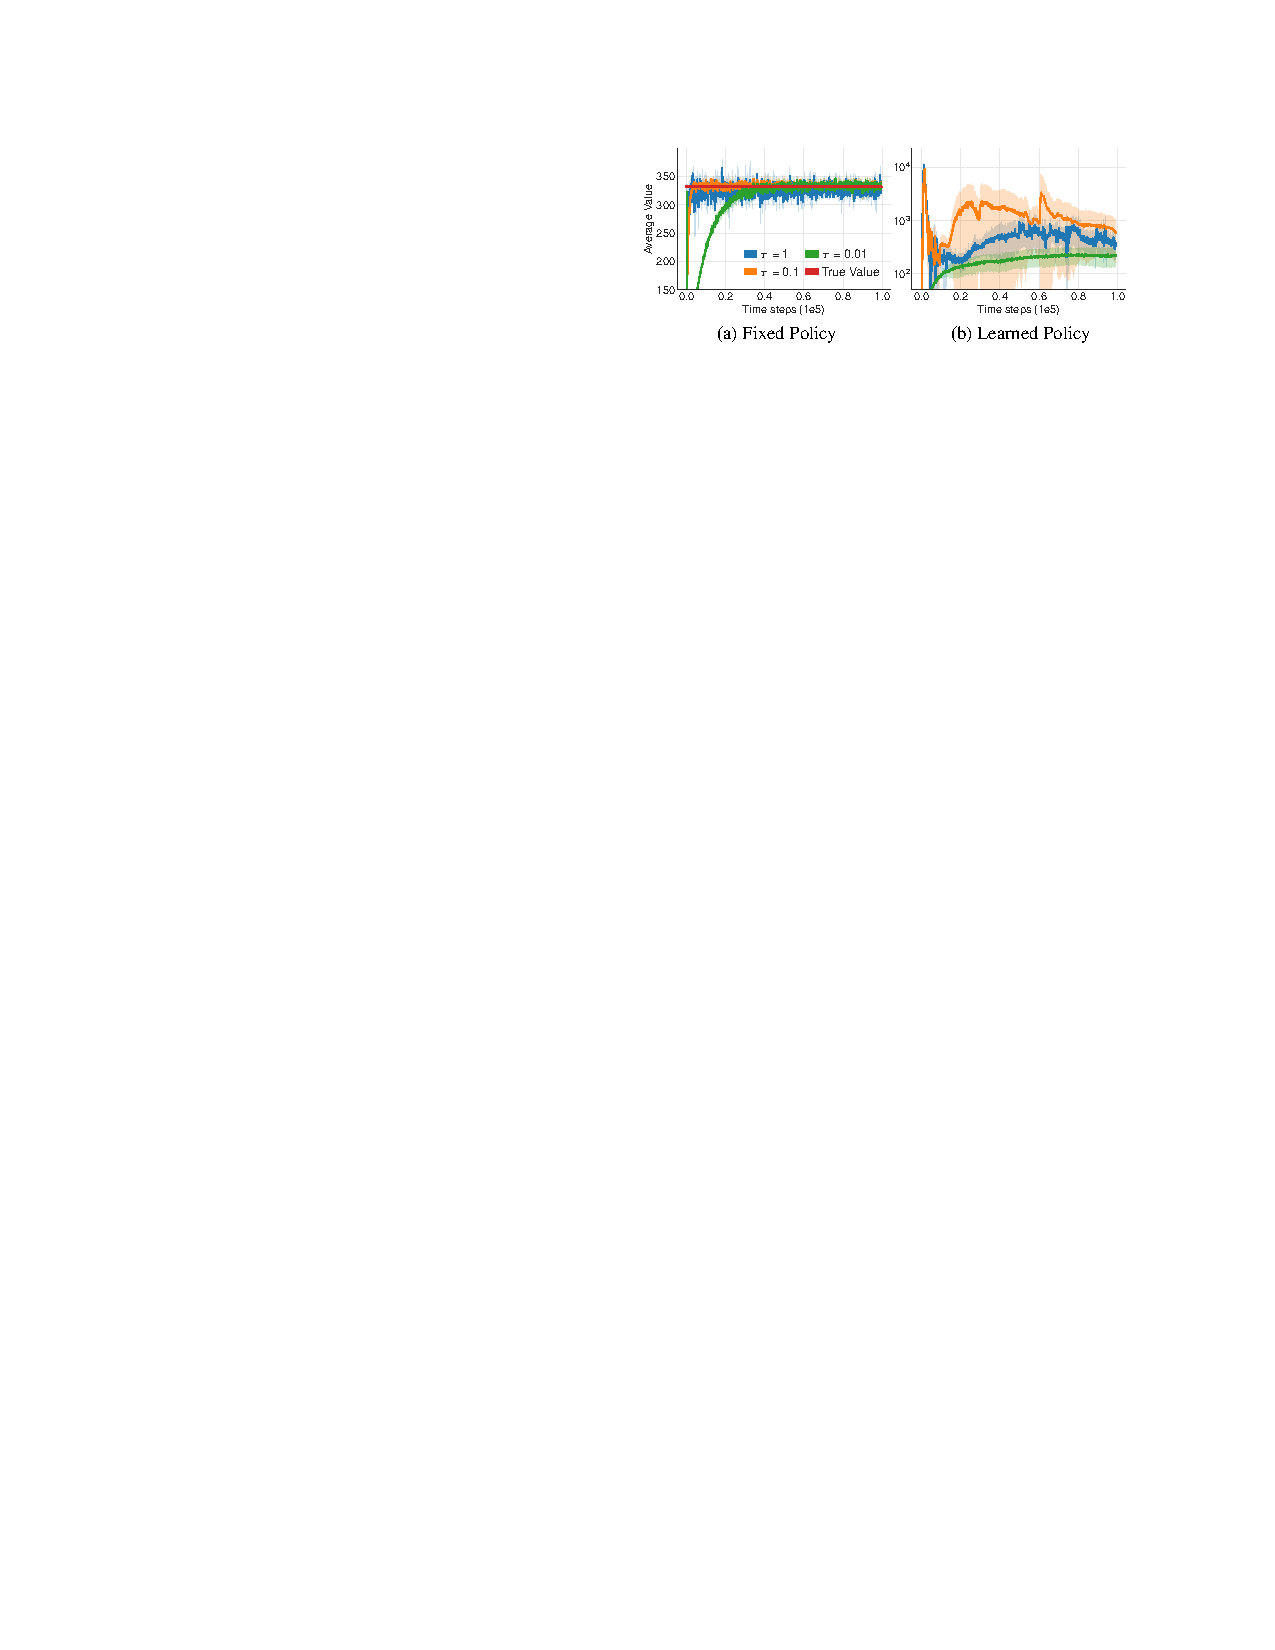
\includegraphics[height=4cm]{fig/lec12/Policy_Update_Frequency_TD3.pdf}
	\caption{Average estimated action value of a randomly selected state on Hopper-v1 environment from \href{https://gym.openai.com/envs/\#mujoco}{OpenAI Gym} (source: S. Fujimoto et al., \textit{Addressing Function Approximation Error in Actor-Critic Methods}, 2018.}
	\label{fig:Policy_Update_Frequency_TD3}
\end{figure}
}	

%%%%%%%%%%%%%%%%%%%%%%%%%%%%%%%%%%%%%%%%%%%%%%%%%%%%%%%%%%%%%
%% Algorithmic Implementation: TD3 %%
%%%%%%%%%%%%%%%%%%%%%%%%%%%%%%%%%%%%%%%%%%%%%%%%%%%%%%%%%%%%%
\frame{%\frametitle{algo. implementation: td3}
\setlength{\algomargin}{0.5em}
\begin{algorithm}[H]
\footnotesize
\SetKwInput{Input}{input} 
\SetKwInput{Output}{output}
\SetKwInput{Init}{init}
\SetKwInput{Param}{parameter}
\Input{diff. deterministic policy function $\bm{\mu}(\bm{x},\bm{\theta})$ and action-value function $\hat{q}(\bm{x},\bm{u},\bm{w})$}
\Param{step sizes and filter constant $\{\alpha_{w}, \alpha_{\theta}, \tau\}\in\left\{\mathbb{R}|0<\alpha, \tau<1\right\}$, policy update rate $k_w\in\left\{\mathbb{N}|1\leq k_w\right\}$, target noise $\bm{\Sigma}\in\mathbb{R}^{m \times m}$ and $\bm{c}\in\mathbb{R}^{m}$}
\Init{weights $\{\bm{w}_{1}=\bm{w}_{1}^{-}$, $\bm{w}_{2}=\bm{w}_{2}^{-}\}\in\mathbb{R}^{\zeta}$,  $\bm{\theta}=\bm{\theta}^{-}\in\mathbb{R}^d$ arbitrarily, memory $\bm{\mathcal{D}}$}\pause
 \For{$j=1,2,\ldots,$ episodes}{
		initialize $\bm{x}_0$\; 
		\For{$k=0,1,\ldots, T-1$ time steps}{
			$\bm{u}_k \leftarrow$ apply from $\bm{\mu}(\bm{x}_k, \bm{\theta})$ w/wo noise or from behavior policy\;
			observe $\bm{x}_{k+1}$ and $r_{k+1}$\;
			store tuple $\left\langle \bm{x}_k, \bm{u}_k, r_{k+1}, \bm{x}_{k+1}\right\rangle$ in $\bm{\mathcal{D}}$\;\pause
			sample mini-batch $\bm{\mathcal{D}}_b$ from $\bm{\mathcal{D}}$ (after initial memory warmup)\;
			\For(calculate $Q$-targets){$i=1,\ldots,b$ samples}{
				\lIf{$\bm{x}_{i+1}$ is terminal}{$y_i=r_{i+1}$}
				\Else{
							$\bm{u}'=\mathrm{clip}\left(\bm{\mu}_{\bm{\theta}^{-}}(\bm{x}_{i+1})+\mathrm{clip}\left(\mathcal{N}(\bm{0},\bm{\Sigma}), -\bm{c},\bm{c}\right), \underline{\bm{u}}, \overline{\bm{u}} \right)$\;	
							$y_i= r_{i+1}+ \gamma \min_{l=1,2}\hat{q}(\bm{x}_{i+1},\bm{u}',\bm{w}_{l}^{-})$\;
							}
			}\pause
			fit $\bm{w}_{l}$ on loss $\mathcal{L}(\bm{w}_{l})=[y - \hat{q}(\bm{x}, \bm{u}, \bm{w}_{l})]^2_{\bm{\mathcal{D}}_b}$ with step size $\alpha_{w}$ $\forall \, l$\;\pause
			\If{$k \mod k_w=0$}{
					$\bm{\theta} \leftarrow \bm{\theta} + \alpha_{\theta} [\nabla_{\bm{\theta}}\bm{\mu}(\bm{x},\bm{\theta})\nabla_{\bm{u}}\hat{q}(\bm{x}, \bm{u}, \bm{w}_1)\vert_{\bm{u}=\bm{\mu}_{\bm{\theta}}(\bm{x})}]_{\bm{\mathcal{D}}_b}$\; \pause
					$\bm{w}_{l}^{-} \leftarrow (1-\tau)\bm{w}_{l}^{-}+\tau\bm{w}_{l}, \,\, \bm{\theta}^{-} \leftarrow (1-\tau)\bm{\theta}^{-}+\tau\bm{\theta}$\;
			}
	}
}
\caption{Twin delayed deep deterministic policy gradient (TD3)}
\label{algo:TD3}
\end{algorithm}
}

%%%%%%%%%%%%%%%%%%%%%%%%%%%%%%%%%%%%%%%%%%%%%%%%%%%%%%%%%%%%%
%% Summary %%
%%%%%%%%%%%%%%%%%%%%%%%%%%%%%%%%%%%%%%%%%%%%%%%%%%%%%%%%%%%%%
\begin{frame}
\frametitle{Summary: what you've learned today}
\begin{itemize}
	\item The deep deterministic policy gradient (DDPG) approach 'transfers' many deep $Q$-network (DQN) ideas to continuous action spaces.\pause
	\item It mainly combines DQN + deterministic policy gradients + policy and value target networks (plus additional minor tweaks).\pause
	\item However, the DDPG actor-critic suffers from value overestimation and high variance during learning. Hence, sampled policy gradients might not be optimal (pointing towards overrated action values).\pause
	\item Twin delayed DDPG (TD3) adds clipped double $Q$-learning, delayed policy updates and target policy smoothing to counteract these issues.
\end{itemize}
\end{frame}
